\section{Path Loss "Free Space Loss vs engineering building space loss"}\label{sc:pathLoss}

To be able to understand the need for relaying, one must first understand the boundaries of the chosen working environment. The range equation gives a nice theoretical reference point to how a far a certain quality signal can be transmitted in optimal conditions. The range equation is dependent on transmission frequency and characteristics of the transmitting and receiving antenna. The frequency dependency comes from the range equation calculation of the far field distance from the antenna pair. The far field distance is when the magnetic and electric part of the signal has a steady state phase relation. Also, the far field distance is dependent on the size and type of the antenna, while the Telosb has a 2.7cm inverted f-antenna and it is transmitting at $2.408GHz$ centre frequency. $2.408GHz$ transmission frequency is chosen from the standard IEEE\_802.15.4, making $2.401GHz$ a ‘1’ and $2.408$ a ‘0’. Trying to keep the frequency as low as possible gives longer transmit range both in theory and in practice, as the lower frequencies have better penetration chances given obstacles. The radiation pattern, $-3dB$ power line, of a Ferrite-based inverted F-antenna can be seen in Figure \ref{fig:invertedAntenna} [6]. Focusing on protocol and power consumption the range equation will be visualized based on an omnidirectional antennas with same polarization, isotropic.


Telosb software specifies transmission power in dBm and the receiving and transmitting antenna have same characterises, so the need to understand the antenna characteristics beyond the far field distance estimation is not needed for this project. Since the main scope of the project is package control protocol, each antenna is treated as an isotropic antenna being able to broadcast up to $100m$ in each direction as specified in the datasheet. To simulate a real scenario the transmitting antenna could be mounted on a rotational motor following the runner through computer vision hence the main beam, e.g. $153\deg$, of the antenna pattern would always point towards the runner verifying our calculation approach. Giving a far field distance of $0.01167m$ and optimal conditions in air, Figure \ref{fig:logpathReceivedSignal_baseStation_air_highSignal} shows the expected received signal strength indication, RSSI, based on the range equation, Equation \ref{eq:rangeEquation} and presumed assumptions.

\begin{figure}[H]
	\centering
	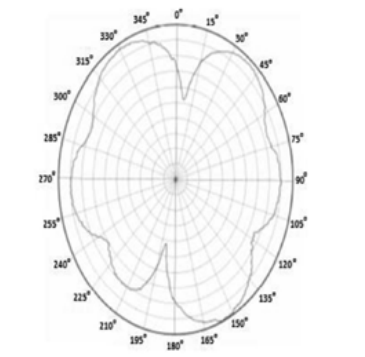
\includegraphics[width=0.8\linewidth]{theory/pathLoss/fig/invertedAntenna.png}
	\caption{Estimation of an inverted F-Antenna radiation pattern.}
	\label{fig:invertedAntenna}
\end{figure}

\clearpage

\begin{figure}[H]
	\begin{flalign*}
		f &= 2.407 \cdot 10^{9} Hz \qquad
		D = 2.7 \cdot 10^{-3} m \\
		\lambda &= \frac{c}{f} = 0.125m \qquad
		\gamma_{air} = 2 \qquad
		\gamma_{building} = 5.5\\
		d{0} &= \frac{2 \cdot D^{2}}{\lambda} = 1.171 \cdot 10^{-4} m
	\end{flalign*}
	
	\begin{subequations}
		\label{eq:rangeEquation}
		\begin{align}
			P_{rcvd}(d) &= \frac{ P_{tx} \cdot G_{t} \cdot G_{r} \cdot \lambda^{2} }{ (4 \pi)^{2} \cdot d^{2} \cdot L }\\
			&= \frac{ P_{tx} \cdot G_{t} \cdot G_{r} \cdot \lambda^{2} }{ (4 \pi)^{2} \cdot d_{0}^{2} \cdot L } \cdot \bigg (\frac{d_{0}}{d} \bigg )^{2}\\
			&= P_{rcvd}(d_{0}) \cdot \bigg (\frac{d_{0}}{d} \bigg )^{\gamma}
		\end{align}
	\end{subequations}
	\caption{Range equation based on a $2.7cm$ wide inverted f-antenna and a $2.408GHz$ center frequency}
\end{figure}

%Figure 3
\begin{figure}[H]
	\centering
	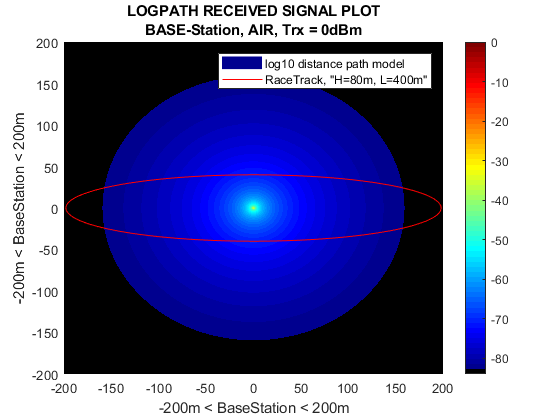
\includegraphics[width=\linewidth]{theory/pathLoss/fig/logpathReceivedSignal_baseStation_air_highSignal.png}
	\caption{$-84dBm$ $159.3m$ received signal area of the race track. The antenna cannot cover the entirety of the racetrack.}
	\label{fig:logpathReceivedSignal_baseStation_air_highSignal}
\end{figure}


Given a racetrack of $400m$ in width, under optimal conditions, as shown in Figure \ref{fig:logpathReceivedSignal_baseStation_air_highSignal}, a telosb will not be able to cover the entirety of the race track and two additional relay “hop” stations must be applied to give sufficient cover. The antenna dimension and transmission power gives a natural boundary to which relaying will be the only option. Figure \ref{fig:logpathReceivedSignal_eachStation_air_highSignal} show the RSSI of the two relay stations in comparison to the base station, while Figure 4 \ref{fig:logpathReceivedSignal_combinedStations_air_highSignal} shows the combined RSSI of the runner node.

%Figure 4
\begin{figure}[H]
	\centering
	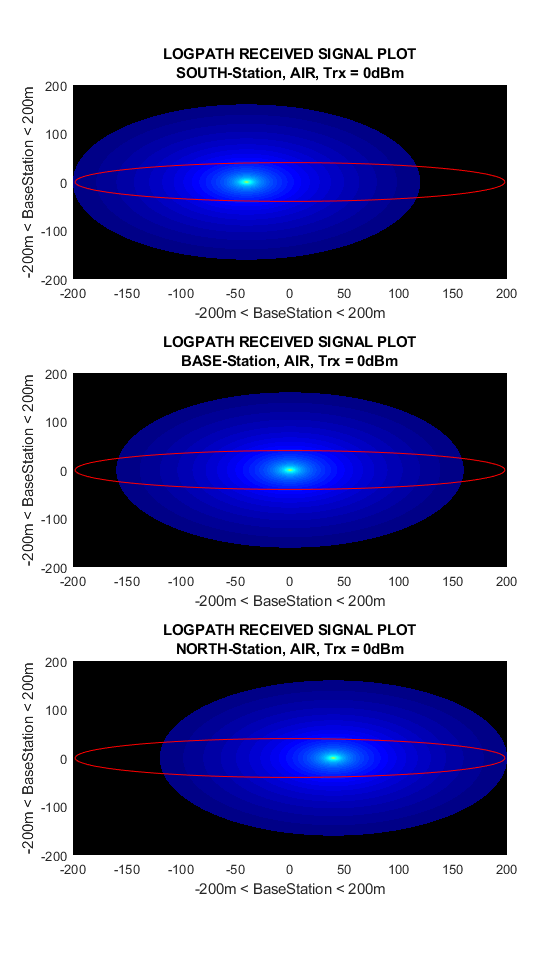
\includegraphics[width=\linewidth]{theory/pathLoss/fig/logpathReceivedSignal_eachStation_air_highSignal.png}
	\caption{Three stations covering the entirety of the racetrack individually.}
	\label{fig:logpathReceivedSignal_eachStation_air_highSignal}
\end{figure}


\begin{figure}[H]
	\centering
	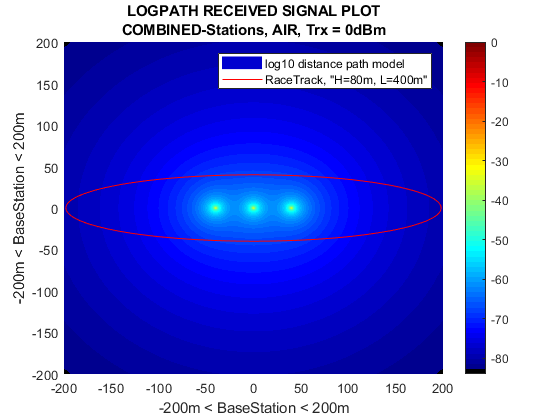
\includegraphics[width=\linewidth]{theory/pathLoss/fig/logpathReceivedSignal_combinedStations_air_highSignal.png}
	\caption{Three stations covering the entirety of the racetrack combined.}
	\label{fig:logpathReceivedSignal_combinedStations_air_highSignal}
\end{figure}

Minimizing the transmission power can lead to extended life time of the individual nodes and the system all together, but at the cost of less coverage area. Figure \ref{fig:logpathReceivedSignal_baseStation_air_lowSignal} shows the single and Figure \ref{fig:logpathReceivedSignal_combinedStations_air_lowSignal} the combined RSSI of the runner node with all nodes using transmission power of $-24dBm$. The size of the race track now is only $7.5\%$ of the full power track. 

%Figure 5
\begin{figure}[H]
	\centering
	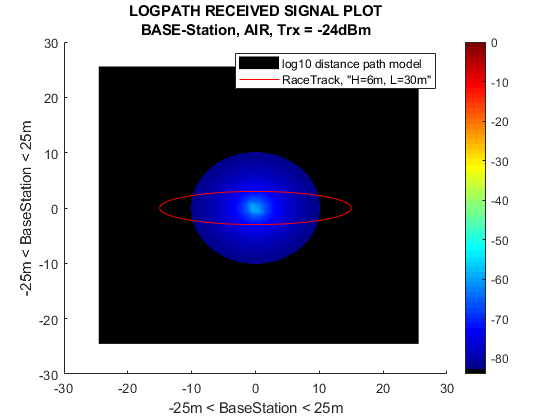
\includegraphics[width=\linewidth]{theory/pathLoss/fig/logpathReceivedSignal_baseStation_air_lowSignal.png}
	\caption{$10.1m$ adequate RSSI for the base station.}
	\label{fig:logpathReceivedSignal_baseStation_air_lowSignal}
\end{figure}

\begin{figure}[H]
	\centering
	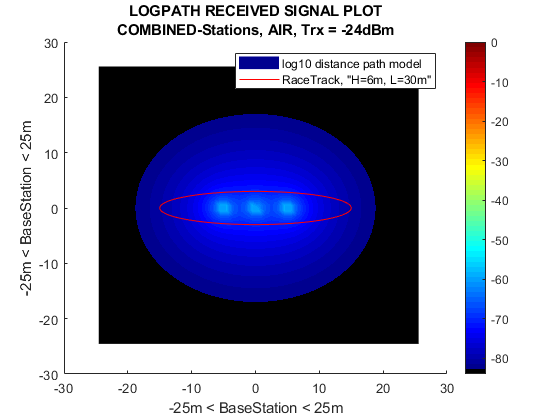
\includegraphics[width=\linewidth]{theory/pathLoss/fig/logpathReceivedSignal_combinedStations_air_lowSignal.png}
	\caption{$10.1m$ Three stations combined RSSI.}
	\label{fig:logpathReceivedSignal_combinedStations_air_lowSignal}
\end{figure}


Further reduction in RSSI can happen for multiple reasons, e.g. reflection, diffraction, scattering and doppler fading. An easy noise model can be to change $\gamma_{air}$ in Equation \ref{eq:rangeEquation} to $\gamma_{building}$, with values taken from page 93 [REF 1]. Figure \ref{fig:logpathReceivedSignal_baseStation_office_lowSignal} and \ref{fig:logpathReceivedSignal_combinedStations_office_lowSignal} shows the distance at minimum Ptr and inside Shannon providing a stunning $0.035\%$ of the coverage related to full power in open AIR.

%Figure 6
\begin{figure}[H]
	\centering
	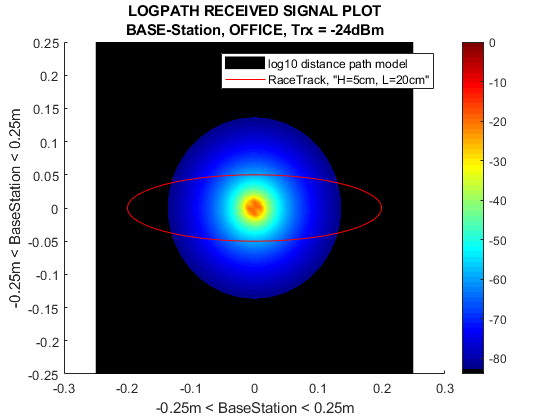
\includegraphics[width=\linewidth]{theory/pathLoss/fig/logpathReceivedSignal_baseStation_office_lowSignal.png}
	\caption{$13.1cm$ adequate RSSI for the base station.}
	\label{fig:logpathReceivedSignal_baseStation_office_lowSignal}
\end{figure}

\begin{figure}[H]
	\centering
	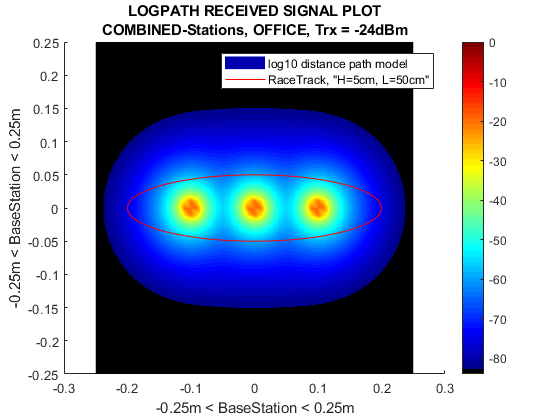
\includegraphics[width=\linewidth]{theory/pathLoss/fig/logpathReceivedSignal_combinedStations_office_lowSignal.png}
	\caption{$13.1cm$ Three stations combined RSSI.}
	\label{fig:logpathReceivedSignal_combinedStations_office_lowSignal}
\end{figure}